% Fig. 1 — Signal-driven 6-route RAG pipeline (Bible_RAG)
% Architecturally faithful to the deployed code as of 2026-05.
% Compile:  pdflatex -interaction=nonstopmode fig1_architecture.tex
% Canvas is fixed to 15.215cm x 10.0cm (aspect 1.5215:1) so the rendered
% PNG drops into the existing <wp:extent> box of biblerag.docx undistorted.
\documentclass[border=0pt]{standalone}
\usepackage{amssymb}
\usepackage{tikz}
\usetikzlibrary{arrows.meta,shapes.geometric}

\begin{document}
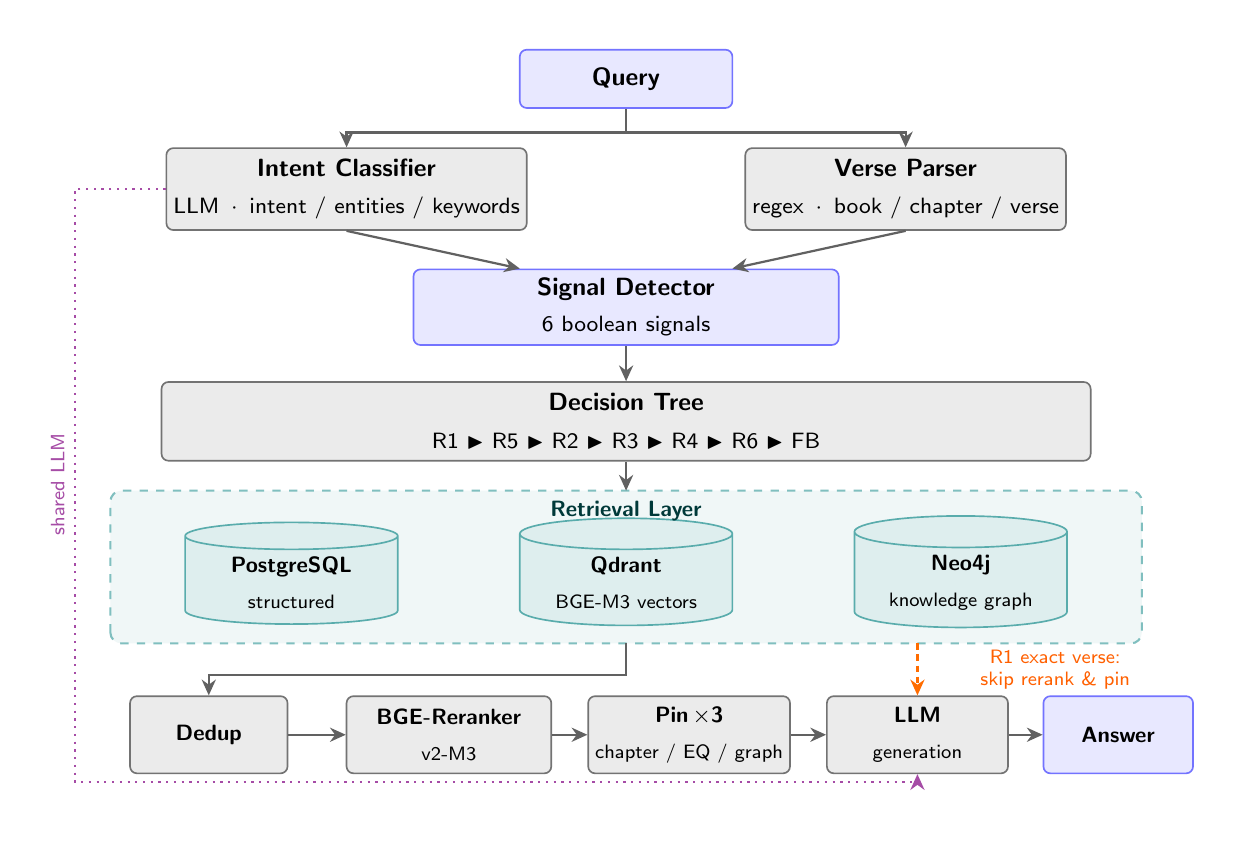
\begin{tikzpicture}[
  font=\sffamily,
  >={Stealth[length=2.0mm,width=1.8mm]},
  stage/.style={rectangle, rounded corners=2.5pt, draw=blue!55, fill=blue!9,
                line width=0.6pt, align=center, inner sep=2.5pt},
  proc/.style={rectangle, rounded corners=2.5pt, draw=black!55, fill=black!8,
               line width=0.6pt, align=center, inner sep=2.5pt},
  db/.style={cylinder, shape border rotate=90, aspect=0.20, draw=teal!65,
             fill=teal!13, line width=0.6pt, align=center, inner sep=2.5pt},
  flow/.style={->, draw=black!62, line width=0.8pt},
  bypass/.style={->, draw=orange!85!red, line width=0.8pt, dashed,
                 dash pattern=on 2.4pt off 1.6pt},
  shared/.style={->, draw=violet!70, line width=0.8pt, dotted},
  lbl/.style={font=\scriptsize\sffamily, inner sep=1pt},
]

% --- fixed bounding box (white background) ---
\fill[white] (0,0) rectangle (15.215,10);

% --- Retrieval Layer container (drawn before the DB nodes so they sit on top) ---
\draw[draw=teal!50, dashed, line width=0.75pt, rounded corners=4pt,
      fill=teal!6] (1.05,2.18) rectangle (14.15,4.12);

% ============================ NODES =================================
% Band 1 -- Query
\node[stage, minimum width=2.7cm, minimum height=0.74cm] (query)
  at (7.6,9.35) {\small\textbf{Query}};

% Band 2 -- Intent Classifier (left) | Verse Parser (right)
\node[proc, minimum width=3.7cm, minimum height=1.04cm] (intent)
  at (4.05,7.95)
  {\small\textbf{Intent Classifier}\\[1.2pt]
   {\footnotesize LLM \,$\cdot$\, intent / entities / keywords}};
\node[proc, minimum width=3.7cm, minimum height=1.04cm] (vparser)
  at (11.15,7.95)
  {\small\textbf{Verse Parser}\\[1.2pt]
   {\footnotesize regex \,$\cdot$\, book / chapter / verse}};

% Band 3 -- Signal Detector
\node[stage, minimum width=5.4cm, minimum height=0.96cm] (signal)
  at (7.6,6.45)
  {\small\textbf{Signal Detector}\\[1.2pt]
   {\footnotesize 6 boolean signals}};

% Band 4 -- Decision Tree (corrected route order)
\node[proc, minimum width=11.8cm, minimum height=1.0cm] (decision)
  at (7.6,5.0)
  {\small\textbf{Decision Tree}\\[1.5pt]
   {\footnotesize R1 $\blacktriangleright$ R5 $\blacktriangleright$ R2
    $\blacktriangleright$ R3 $\blacktriangleright$ R4 $\blacktriangleright$
    R6 $\blacktriangleright$ FB}};

% Band 5 -- Retrieval Layer container + 3 databases
\node[db, minimum width=2.7cm, minimum height=1.2cm] (pg)
  at (3.35,2.95) {\footnotesize\textbf{PostgreSQL}\\[1pt]{\scriptsize structured}};
\node[db, minimum width=2.7cm, minimum height=1.2cm] (qd)
  at (7.6,2.95) {\footnotesize\textbf{Qdrant}\\[1pt]{\scriptsize BGE-M3 vectors}};
\node[db, minimum width=2.7cm, minimum height=1.2cm] (n4)
  at (11.85,2.95) {\footnotesize\textbf{Neo4j}\\[1pt]{\scriptsize knowledge graph}};
\node[font=\footnotesize\sffamily, text=teal!45!black]
  at (7.6,3.86) {\textbf{Retrieval Layer}};

% Band 6 -- post-retrieval chain: Dedup -> Reranker -> Pin -> LLM -> Answer
\node[proc, minimum width=2.0cm, minimum height=0.98cm] (dedup)
  at (2.30,1.02) {\footnotesize\textbf{Dedup}};
\node[proc, minimum width=2.6cm, minimum height=0.98cm] (rerank)
  at (5.35,1.02) {\footnotesize\textbf{BGE-Reranker}\\[1pt]{\scriptsize v2-M3}};
\node[proc, minimum width=2.5cm, minimum height=0.98cm] (pin)
  at (8.40,1.02) {\footnotesize\textbf{Pin\,$\times$3}\\[1pt]{\scriptsize chapter / EQ / graph}};
\node[proc, minimum width=2.3cm, minimum height=0.98cm] (llm)
  at (11.30,1.02) {\footnotesize\textbf{LLM}\\[1pt]{\scriptsize generation}};
\node[stage, minimum width=1.9cm, minimum height=0.98cm] (answer)
  at (13.85,1.02) {\footnotesize\textbf{Answer}};

% ============================ EDGES =================================
% main flow
\draw[flow] (query.south) -- ++(0,-0.30) -| (intent.north);
\draw[flow] (query.south) -- ++(0,-0.30) -| (vparser.north);
\draw[flow] (intent.south)  -- ([xshift=-1.35cm]signal.north);
\draw[flow] (vparser.south) -- ([xshift=1.35cm]signal.north);
\draw[flow] (signal.south) -- (decision.north);
\draw[flow] (decision.south) -- (7.6,4.12);
\draw[flow] (7.6,2.18) -- ++(0,-0.40) -| (dedup.north);
\draw[flow] (dedup.east)  -- (rerank.west);
\draw[flow] (rerank.east) -- (pin.west);
\draw[flow] (pin.east)    -- (llm.west);
\draw[flow] (llm.east)    -- (answer.west);

% R1 exact-verse bypass: skips Reranker + Pin, straight to the LLM
\draw[bypass] (11.30,2.18) -- (llm.north);
\node[lbl, text=orange!75!red, align=center] at (13.05,1.85)
  {R1 exact verse:\\skip rerank \& pin};

% Shared LLM: the intent classifier and the generator are one model
\draw[shared] (intent.west) -- (0.60,7.95) -- (0.60,0.42)
              -- (11.30,0.42) -- (llm.south);
\node[lbl, text=violet!70, rotate=90] at (0.38,4.2) {shared LLM};

\end{tikzpicture}
\end{document}
